\documentclass[11pt, oneside]{amsart}   	% use "amsart" instead of "article" for AMSLaTeX format
\usepackage[top=0.3cm, bottom=1.3cm, left=1cm, right=1cm]{geometry}                		% See geometry.pdf to learn the layout options. There are lots.
\geometry{letterpaper}                   		% ... or a4paper or a5paper or ... 
%\geometry{landscape}                		% Activate for rotated page geometry
%\usepackage[parfill]{parskip}    		% Activate to begin paragraphs with an empty line rather than an indent
\usepackage{graphicx}				% Use pdf, png, jpg, or eps§ with pdflatex; use eps in DVI mode
\usepackage{bm}							% TeX will automatically convert eps --> pdf in pdflatex		
\usepackage{amssymb}
\usepackage{amsmath}
\usepackage{subcaption}
\usepackage{float}
\pagenumbering{gobble}


\title{MVA-DM3 Probabilistic graphical models}
\author{Hugo Cisneros}
\date{}							% Activate to display a given date or no date

\begin{document}
\maketitle
\section{Implementation - HMM}
\textbf{1.2} For a set of parameters $\theta$ in the Gaussian Mixture Hidden Markov model (GM-HMM), the complete likelihood can be written:
\begin{align*}
	l_c(\theta) &= \log\left(p(q_0)\prod_{t=0}^{T-1} p(q_{t+1}|q_t) \prod_{t=0}^T p(\overline{y}_t|q_t)\right)\\
		&= \sum_{i=1}^K \delta(q_0 = i)\log(\pi_i) + \sum_{t=0}^{T-1}\sum_{i,j=1}^K\delta(q_{t+1}=i, q_t=j)\log(A_{i,j})+  \sum_{t=0}^{T}\sum_{i=1}^K \delta(q_t = i) \log \mathcal{N}(\overline{y}_t|\mu_t, \Sigma_t)
\end{align*}
 For the EM algorithm, we wish to compute the parameters of the HMM with the observations $(\overline{y}_t)$. A lower bound of the likelihood is found by using Jensen's inequality with the $\log$ function, which gives $ \log p(\overline{y}_0, ..., \overline{y}_T) \geq \mathbb{E}_q[l_c(\theta)]$. 
 
 We use the notations $\gamma(q_t)_i = p(q_t = i | \overline{y}, \theta)$ and $\xi(q_{t+1}, q_t)_{ij} = p(q_{t+1}=i, q_t=j |  \overline{y}, \theta)$. The expression $ \mathbb{E}_q[l_c(\theta)]$ becomes 
 \[
 \mathbb{E}_q[l_c(\theta)] = \sum_{i=1}^K\gamma(q_0)_i\log(\pi_i) + \sum_{t=0}^{T-1}\sum_{i,j=1}^K\xi(q_{t+1}, q_t)_{ij}\log(A_{i,j})+  \sum_{t=0}^{T}\sum_{i=1}^K\gamma(q_t)_i \log \mathcal{N}(\overline{y}_t|\mu_t, \Sigma_t)
 \]
 By maximizing w.r.t $\pi$ and $A$ we get $\boxed{\pi_i = \dfrac{\gamma(q_0)_i}{\sum_{j=1}^K\gamma(q_0)_j}}$ and $\boxed{A_{i,j} = \dfrac{\sum_{t=0}^{T-1}\xi(q_{t+1}, q_t)_{ij}}{\sum_{i=1}^K \sum_{t=0}^{T-1}\xi(q_{t+1}, q_t)_{ij}}}$. The other derivations are similar to the ones from the Gaussian Mixture model in Homework 2. 
 \\
 
 We have : $\boxed{\mu_i = \dfrac{\sum_{t=0}^T \gamma(q_t)_i \overline{y}_t}{\sum_{t=0}^T \gamma(q_t)_i}}$ and $\boxed{\Sigma_i = \dfrac{\sum_{t=0}^{T}  \gamma(q_t)_i  (\overline{y}_t - \mu_i)(\overline{y}_t - \mu_i)^T}{\sum_{t=0}^T \gamma(q_t)_i}}$ weighted sums of the empirical means and covariances.
 \begin{figure}[!h]
 \centering
 \begin{subfigure}{.4\textwidth}
 \centering
  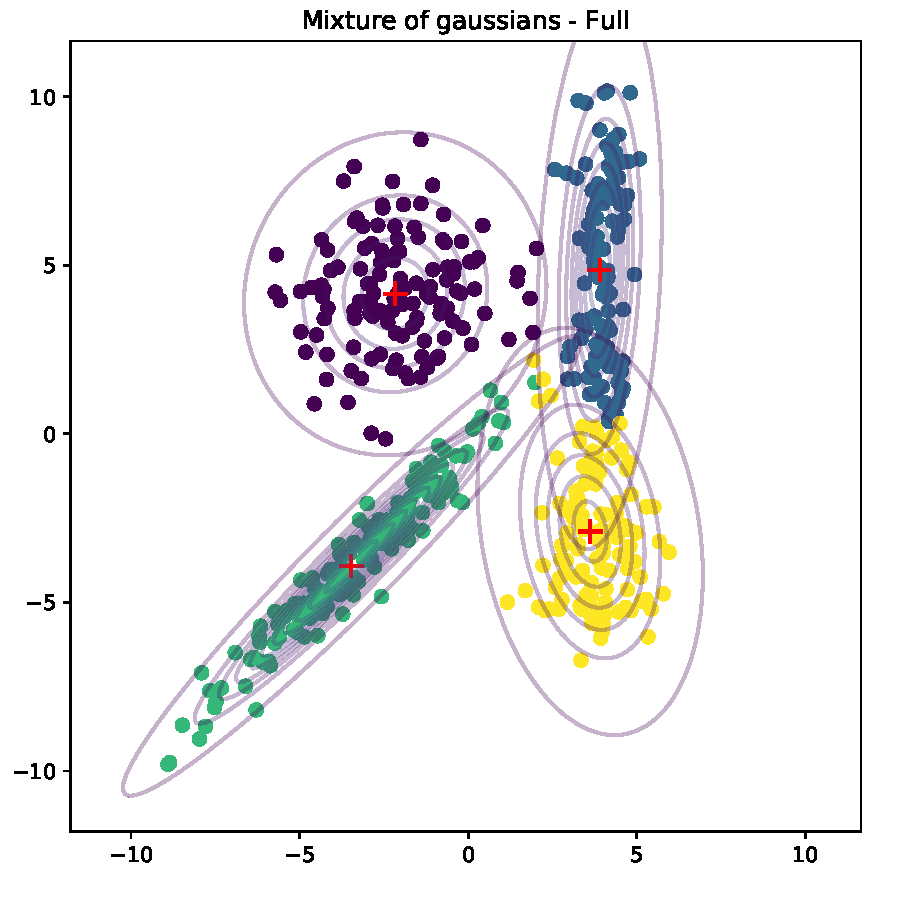
\includegraphics[width=.8\linewidth]{full.pdf}
  \caption{Gaussian mixture}
 \end{subfigure}
   \begin{subfigure}{.4\textwidth}
    \centering
 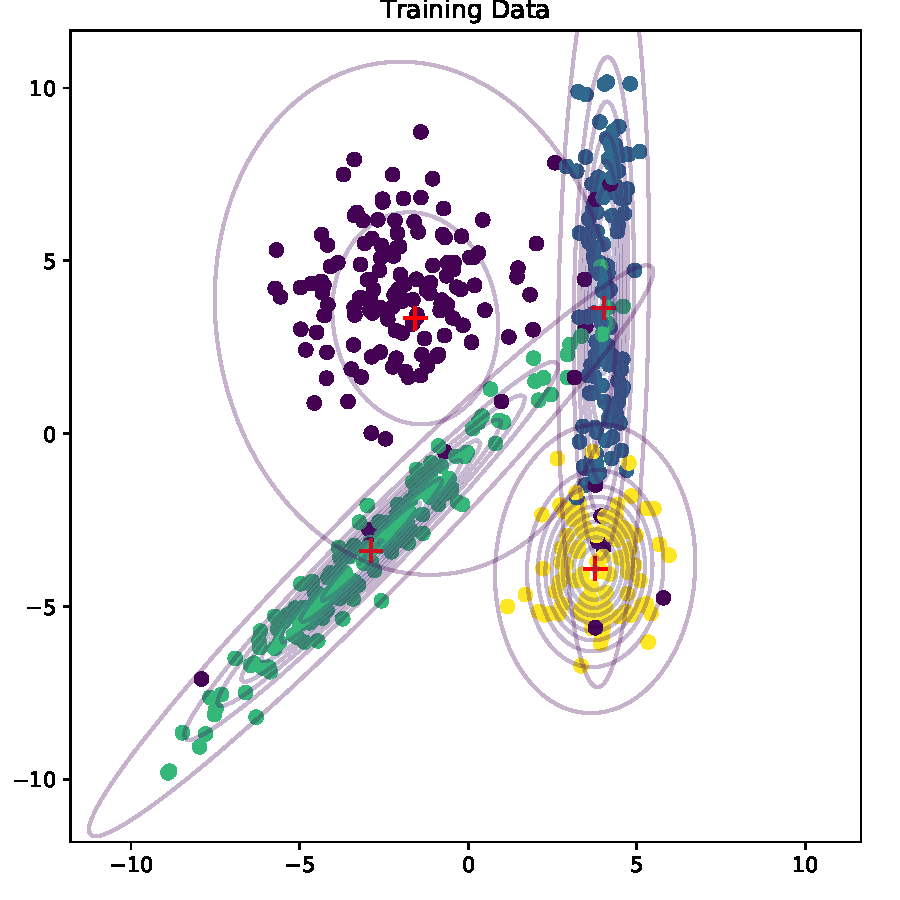
\includegraphics[width=.8\linewidth]{training_gmhmm.pdf}
 \caption{GM-Hidden markov model}
 \end{subfigure}
 \caption{Comparison of mixture of gaussian profile and cluster assignment (most probable sequence of hidden state for HMM) for the Gaussian mixture model and GM-HMM.}
 \end{figure}
 
 \textbf{1.5} The GM-HMM learns a slightly different mixture configuration than the GM model. The assumption that data is temporally distributed is strong and yields some artifacts such as outliers assigned to a very unlikely hidden state. However, the likelihood on both training data and test data is much higher than for the Gaussian mixtrure:  -2101.4 and -2201 for GM-HMM against -2340.2 for the training set and -2431 for the test set for the GM model.
 
 \end{document}